% Estas slides tienen que abrirse con el programa pdfpc que soporta videos embebidos
% el comando es: pdfpc -g slides.pdf
% para los videos se requiere ubuntu-restricted-extras
% para la bibliografía se requiere biber y configurar texstudio

%\documentclass[compress,handout]{beamer}
\documentclass[aspectratio=169,compress]{beamer}

% add beamer preamble
% In this preamble should go only package and settings related with beamer

% Theme customization
\setbeamertemplate{itemize item}[rectangle] % configure itemize
\setbeamertemplate{itemize subitem}[circle] % configure itemize
\setbeamertemplate{itemize subsubitem}[triangle] % configure itemize
\setbeamertemplate{navigation symbols}{} % remover simbolos de navegacion de las slides
\usefonttheme[onlymath]{serif} % simbolos matematicos en serif (Como es en latex original)
\setbeamersize{text margin left=3mm,text margin right=3mm} 

\setbeamertemplate{blocks}[rounded] % blocks corners rounded
\setbeamercolor{block body}{bg=blue!12,fg=black} % color of blocks
\setbeamertemplate{caption}{\raggedright\insertcaption\par} % elimina la palabra "Figura" del caption

\usepackage[overridenote]{pdfpc} % requires to download manually pdfpc.sty package from https://www.ctan.org/pkg/pdfpc


% HOW TO SHOW ADDITIONAL SLIDES%
\newif\ifadditional % conditional to show additional slides
%\additionaltrue   % uncomment to show additional slides
\additionalfalse % uncomment to show without additional slides

% Reference cite without footnote mark
\newrobustcmd*{\footfullcitenomark}{%
    \AtNextCite{%
        \let\thefootnote\relax
        \let\mkbibfootnote\mkbibfootnotetext}%
    \footfullcite}


% add latex preamble
% para la bibliografía se requiere biber y configurar texstudio

% Latex packages
\usepackage[utf8]{inputenc}
\usepackage[T1]{fontenc} % para copiar acentos en español del pdf y permite acentos en las notas
\usepackage[spanish]{babel}
\usepackage[per-mode = symbol]{siunitx} % para manejar las unidades
\usepackage{multimedia} % to add videos with \movie command
\usepackage{multirow}
\usepackage{graphicx}
\usepackage{xcolor}
\usepackage{amsmath} % bmatrix
\usepackage[makeroom]{cancel} % \cancel to cancel terms in math equations
\renewcommand{\CancelColor}{\color{red}} % set red color for \cancel command
\usepackage[caption=false]{subfig} % caption = false elimina la palabra "Figura" del caption
\usepackage{import} % para el comando import (se usa para pdf_tex)
\captionsetup[subfigure]{labelformat=empty} % remover el indice del caption de la subfigura
\usepackage{booktabs} % \toprule \midrule \bottomrule
\usepackage[backend=biber]{biblatex} % set biber to format references. Must configure Biber in Texstudio
\usepackage{csquotes} % to remove warning triggered by biblatex and babel
\usepackage{algpseudocode} % to write algorithm
\usepackage{tikz} % to use tikz
\usepackage[export]{adjustbox} %valign in subfloat
\usepackage{colortbl} % to paint cells in a table

% Color commands for annotations
\newcommand\TODO[1]{\textbf{\textcolor{red}{#1}}} %  TODO notes

% Graphic paths
\graphicspath{{./images/}}

% listings configuration for C code
\usepackage{listings} % code
\definecolor{commentgreen}{RGB}{2,112,10}
\definecolor{eminence}{RGB}{108,48,130}
\definecolor{weborange}{RGB}{255,165,0}
\definecolor{frenchplum}{RGB}{129,20,83}

\lstset{ % spanish characters for listings package
	inputencoding=latin1,
    columns=fullflexible,
	breaklines=true,
	tabsize=2,
	showstringspaces=false,
	basicstyle=\ttfamily,
	backgroundcolor=\color{lightgray}, % Choose background color
	literate={á}{{\'a}}1
	{ã}{{\~a}}1
	{é}{{\'e}}1
	{ó}{{\'o}}1
	{í}{{\'i}}1
	{ñ}{{\~n}}1
	{¡}{{!`}}1
	{¿}{{?`}}1
	{ú}{{\'u}}1
	{Í}{{\'I}}1
	{Ó}{{\'O}}1
    {-}{-}1
}

\lstdefinestyle{cpp}{ % spanish characters for listings package
    language=C++,
   	commentstyle=\color{commentgreen},
    keywordstyle=\color{eminence},
    stringstyle=\color{red},
    emph={int,char,double,float,unsigned,void,bool},
    emphstyle={\color{blue}}
}

\lstdefinestyle{bash}{ % spanish characters for listings package
	language=Bash
}

\lstdefinestyle{xml}{
	language=XML,
	morekeywords={encoding,xs:schema,xs:element,xs:complexType,xs:sequence,xs:attribute}
}

\lstdefinestyle{cmake}{
	language=make, % there is no cmake support in listings
}

\lstdefinestyle{python}{
    language=python,
}


%%%%% PARA QUE EN LAS TABLAS SE PUEDA PONER UN SALTO DE LINEA DENTRO DE UNA CELDA
\newcommand{\specialcell}[2][c]{%
    \begin{tiny}
        \begin{tabular}[#1]{@{}c@{}}#2\end{tabular}  
    \end{tiny}
}
%%%%%%%%%%%%%%%%%%%%%%%%%%%%%%%%%%%%%%%%%%%%%%%%%%%%%%%%%%%%%%%%%%%%%%%%

%%%%% PARA QUE LAS TABLAS TENGAN TODAS LAS COLUMNAS CENTRADAS Y DE IGUAL TAMAÑO
\usepackage{tabularx}
\renewcommand{\tabularxcolumn}[1]{>{\centering\arraybackslash}m{#1}}
%%%%%%%%%%%%%%%%%%%%%%%%%%%%%%%%%%%%%%%%%%%%%%%%%%%%%%%%%%%%%%%%%%%%%%%%



% add math preamble
\usepackage{amsmath}
\usepackage{amssymb}
\usepackage{amsopn}
\usepackage{mathtools}
\usepackage{nicematrix} % Add colors to matrix


% set matrix maximum length
\setcounter{MaxMatrixCols}{20}

% math
\renewcommand{\vec}[1]{\boldsymbol{\mathbf{#1}}}
\newcommand{\norm}[1]{\lVert#1\rVert}

% Declare arg max and arg min functionss
\DeclareMathOperator*{\argmax}{arg\,max}
\DeclareMathOperator*{\argmin}{arg\,min}

% Declare atan2 
\DeclareMathOperator{\atantwo}{atan2}

% Homogeneous decoration function
\newcommand{\homo}[1]{\dot{#1}}


% Declare projection as math function
\DeclareMathOperator{\proj}{proj}
\newcommand{\fromCoord}[2]{{#1}_\mathrm{#2}}
\newcommand{\toCoord}[2]{\prescript{\mathrm{#2}}{}{#1}}
\newcommand{\worldCoordSystem}{\mathrm{W}}
\newcommand{\bodyCoordSystem}{\mathrm{B}}
\newcommand{\cameraCoordSystem}{\mathrm{C}}
\newcommand{\origin}{\vec{o}}
\newcommand{\point}{\vec{p}}
\newcommand{\worldPoint}{\toCoord{\point}{\worldCoordSystem}}
\newcommand{\imagePoint}{\vec{u}}
\newcommand{\cameraPoint}{\toCoord{\point}{\cameraCoordSystem}}
\newcommand{\homoWorldPoint}{\toCoord{\homo{\point}}{\worldCoordSystem}}
\newcommand{\homoImagePoint}{\homo{\imagePoint}}
\newcommand{\homoCameraPoint}{\toCoord{\homo{\point}}{\cameraCoordSystem}}
\newcommand{\measurement}{\vec{z}}
\newcommand{\prediction}{\hat{\vec{z}}}
\newcommand{\seMatrix}{\vec{\xi}}
\newcommand{\transform}[2]{\toCoord{\fromCoord{\seMatrix}{#2}}{#1}}
\newcommand{\pointCoord}[1]{\toCoord{\point}{#1}}
\newcommand{\rotation}{\vec{R}}
\newcommand{\rotationCoord}[2]{\toCoord{\fromCoord{\rotation}{#2}}{#1}}
\newcommand{\translation}{\vec{t}}
\newcommand{\translationCoord}[2]{\toCoord{\fromCoord{\translation}{#2}}{#1}}
\newcommand{\intrinsicMatrix}{\vec{K}}
\newcommand{\principalPoint}{\vec{c}}
\newcommand{\reprojectionError}{u}
\newcommand{\projectionMatrix}{\vec{P}}
\newcommand{\cameraCenter}{\vec{o}}
\newcommand{\worldCameraCenter}{\toCoord{\cameraCenter}{\worldCoordSystem}}
\newcommand{\essentialMatrix}{\vec{E}}
\newcommand{\fundamentalMatrix}{\vec{F}}
\newcommand{\inverse}[1]{{#1}^{-1}}
\newcommand{\epipole}{\vec{e}}

% Localization (State Estimation)
\newcommand{\state}{x}
\newcommand{\observation}{z}
\newcommand{\controlCommand}{u}
\newcommand{\covariance}{\Sigma}
\newcommand{\motionModelNoise}{\epsilon}
\newcommand{\measurementModelNoise}{\delta}
\newcommand{\motionModelFunction}[1]{g\left( #1 \right)}
\newcommand{\observationModelFunction}[1]{h\left( #1 \right)}
\newcommand{\motionParametersCovariance}{R}
\newcommand{\observationModelCovariance}{Q}
\newcommand{\motionModelJacobian}{G}
\newcommand{\observationModelJacobian}{H}
\newcommand{\kalmanGain}{K}
\newcommand{\normalDistribution}[2]{\mathcal{N}\left( {#1}, {#2} \right)}
\newcommand{\motionModelJacobianControl}{V}
\newcommand{\motionModelCovariance}{M}
\newcommand{\stateEvolutionMatrix}{A}

% Mapping slides
\newcommand{\map}{m}
\newcommand{\mapRandomVariable}{m}

% SLAM slides
\newcommand{\informationMatrix}{\vec{\Omega}}
\newcommand{\error}{\vec{e}}
\newcommand{\observationBold}{\vec{z}}
\newcommand{\stateBold}{\vec{x}}
\newcommand{\jacobian}{\vec{J}}
\newcommand{\linearSystemb}{\vec{b}}
\newcommand{\linearSystemH}{\vec{H}}
\newcommand{\covarianceBold}{\vec{\covariance}}


% Motion Planning slides
\newcommand{\workSpace}{\mathcal{W}}
\newcommand{\obstaclesSet}{\mathcal{O}}
\newcommand{\robotInConfiguration}{\mathcal{A}}
\newcommand{\robotConfiguration}{q}
\newcommand{\configurationSpace}{\mathcal{C}}
\newcommand{\freeConfigurationSpace}{\configurationSpace_{free}}
\newcommand{\obstableConfigurationSpace}{\configurationSpace_{obs}}
\newcommand{\goalSet}{\configurationSpace_{goal}}
\newcommand{\startConfiguration}{\robotConfiguration_{I}}
\newcommand{\goalConfiguration}{\robotConfiguration_{G}}
\newcommand{\continuousPath}{\tau}
\newcommand{\motionLaw}{\gamma}
\newcommand{\robotActionSpace}{\mathcal{U}}


% Motion model
\newcommand{\position}{\vec{p}}
\newcommand{\orientation}{\vec{O}}
\newcommand{\orientationQuaternion}{\vec{q}}
\newcommand{\predictedPosition}{\hat{\vec{p}}}
\newcommand{\predictedOrientationQuaternion}{\hat{\vec{q}}}
\newcommand{\linearVelocity}{\vec{v}}
\newcommand{\angularVelocity}{\vec{\omega}}

\DeclareMathOperator{\slerpOp}{slerp}
\newcommand{\slerp}[1]{\slerpOp{\left( #1 \right)}}

% Map structure
\newcommand{\keyframesSet}{K}
\newcommand{\mapPointsSet}{P}
\newcommand{\observedMapPoints}{O}
\newcommand{\covisibilityKeyframes}{CK}
\newcommand{\localMap}{local\_map}

% Bundle Adjutment
\newcommand{\update}{\vec{\delta}}
\newcommand{\incremental}{\hat{\update}}


% Loop Closure names

% scaled operators and letters to fancy view
\newcommand{\sminus}{\scalebox{0.5}[1.0]{$-$}}
\newcommand{\splus}{\scalebox{0.6}[0.6]{$+$}}
\newcommand{\curr}{c}
\newcommand{\sind}[1]{\scalebox{0.6}[0.6]{$#1$}}
\newcommand{\ind}[1]{\scalebox{0.7}[0.7]{$#1$}}

\newcommand{\keyframe}{\vec{K}}
\newcommand{\bowVector}{\vec{v}}
\newcommand{\lcError}{\vec{\Omega}}
\newcommand{\relativeTransformation}{\seMatrix}
\DeclareMathOperator{\interpolate}{interpolate}

\newcommand{\relativeMotion}{\vec{\delta}}
\newcommand{\groundTruth}[1]{{#1}^{*}}

% definición del operador rot()
\DeclareMathOperator{\rotationOp}{rot}
\newcommand{\getRotation}[1]{\rotationOp{\left( #1 \right)}}

\DeclareMathOperator{\translationOp}{trans}
\newcommand{\getTranslation}[1]{\translationOp{\left( #1 \right)}}









% add bibliography resource
\renewcommand*{\bibfont}{\footnotesize} % change bibliograhy size
\bibliography{../../common/bibliography.bib}

\subtitle{Visión por computadora}
\title{Robótica Móvil}
\author{Taihú Pire}
\institute{Laboratorio de Robótica}
\titlegraphic{
\includegraphics[width=0.4\textwidth]{images/cifasis_logo.pdf}}
\date{}

\begin{document}
	
	% add title page
	\frame{\titlepage}
	
\section{Visión por computadora}
\begin{frame}
	\frametitle{Detección de Keypoints}
	
	\note{https://youtu.be/ebMyBbkkHWk}
	
	\footnotesize
	Propiedades deseables para SLAM / SfM:
	\begin{itemize}
		\item Alta repetitibilidad
		\item Alta precisión
		\item Robustez
		\item Invarianza (luminosidad, puntos de vista, etc)
		\item Computacionalmente eficientes
		\item Algunos detectores: HARRIS, SIFT, SURF, Shi-Tomasi, FAST, ORB, BRISK
	\end{itemize}

	
	\begin{figure}
		\includegraphics[width=0.5\textwidth]{./images/keypoints_fast}
		\caption{Keypoints FAST}
	\end{figure}

\end{frame}


\begin{frame}
	\frametitle{Matcheo de keypoints}
	\footnotesize
	Propiedades deseables del matcheo de keypoints para SLAM / SfM:
	\begin{itemize}
		\item Alto recall
		\item precisión
		\item Robustez
		\item Computacionalmente eficientes
		\item Posibles enfoques: patches o descriptores
	\end{itemize}
	
	\begin{figure}
		\includegraphics[width=0.4\textwidth]{./images/matching_notredam.jpg}
		\caption{Keypoints Harris + Descriptor SIFT}
	\end{figure}
	\note{Imagen extraida de https://www.cc.gatech.edu/classes/AY2016/cs4476_fall/results/proj2/html/cpolack6/index.html}
\end{frame}

\begin{frame}
	\frametitle{Precision - Recall}
	\footnotesize
	
	\note{https://upload.wikimedia.org/wikipedia/commons/2/26/Precisionrecall.svg}
	
	\begin{figure}
		\includegraphics[width=0.25\textwidth]{./images/precision_recall.pdf}
	\end{figure}
\end{frame}

\begin{frame}
	\frametitle{Desciptores de features Locales}
	\footnotesize
	
	Propiedades deseables para SLAM / SfM: distinguibles, robustos, invariantes
	\begin{itemize}
		\item Extraer firmas sobre regiones de la imagen ejemplos:
		\begin{itemize}
			\item Histogramas sobre gradientes de la imagen (SIFT)
			\item Histogramas sobre respuestas Haar-wavelet (SURF)
			\item Patrones binarios (BRIEF, BRISK, FREAK, ORB)
			\item Descriptores basados en aprendizaje
		\end{itemize}
		\item Invariante rotación: Alineado con la orientación dominante de la región local
		\item Invariante a escala: Adaptar la región descripta a la escala de keypoint
	\end{itemize}

	\TODO{agregar imagenes SIFT BRIEF}
	
\end{frame}

\begin{frame}
	\frametitle{Local Features invariantes}
	\footnotesize
	
	\begin{itemize}
		\item Invarianza geométrica: traslación, rotación, escala.
		\item Invarianza fotométrica: brillo, exposición, etc.
	\end{itemize}
	 

\end{frame}

\begin{frame}
	\frametitle{Ventajas de features locales}
	\footnotesize

	\begin{itemize}
	\item Locales: los features al ser locales son robustos a oclusiones
	\item Distintivos: pueden diferenciar un gran conjunto de objetos
	\item Cuantiosos: puede haber cientos o miles en una misma imagen
	\item Eficientes: al discretizar la imagen, se puede obtener tiempo real.
\end{itemize}
	
\end{frame}

\begin{frame}
	\frametitle{Harris}
	\footnotesize
	
	\TODO{Agregar slides de SIFT, HARRIS, FAST y ORB https://youtu.be/ebMyBbkkHWk}
	
\end{frame}

\begin{frame}
	\frametitle{Matcheo de keypoints}
	\footnotesize
	
\end{frame}

\begin{frame}
	\frametitle{RANSAC: Random Sample Consensus}
	\footnotesize
	
	\begin{itemize}
		\item Permite encontrar un modelo que ajusta datos en presencia de ruido y outliers
		\item Separa el conjunto de datos entre inliers y outliers
%		\item Encuentra la mejor partición de puntos en un conjunto de inliers y outliers. Estima un modelo utilizando el conjunto de inliers.
		\item Ejemplo: dado un conjunto de puntos 2D, ajustar una línea 
	\end{itemize}
	
	\begin{figure}
		\includegraphics[width=0.5\textwidth]{./images/ransac_points.pdf}
	\end{figure}

	\TODO{hacer imágenes similares a las del vídeo: https://youtu.be/ebMyBbkkHWk}
	
\end{frame}


\begin{frame}
	\frametitle{RANSAC: Random Sample Consensus}
	\footnotesize
	
	\TODO{hacer imágenes similares a las del vídeo: https://youtu.be/ebMyBbkkHWk}
	
	\begin{figure}
		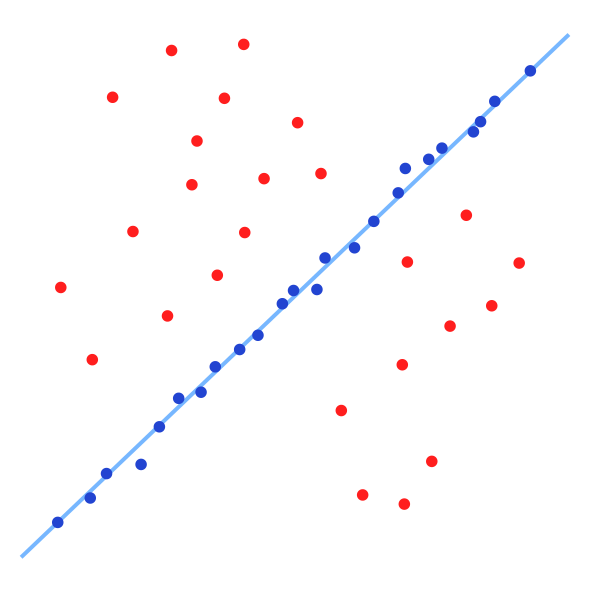
\includegraphics[width=0.5\textwidth]{./images/ransac_fitted_line.pdf}
	\end{figure}
	
\end{frame}
\begin{frame}
	\frametitle{RANSAC: Random Sample Consensus}
	\footnotesize

	\begin{enumerate}
		\item {\bf Samplear} de manera aleatoria el número de puntos requerido para ajustar el modelo.
		\item {\bf Computar} el modelo usando los datos sampleados
		\item {\bf Contar} el número de inliers y quedarse con el modelo que mejor ajusta los datos
		\item Iterar puntos 1-3 hasta que el mejor modelo es hallado
	\end{enumerate}

\end{frame}

\begin{frame}
	\frametitle{RANSAC: Random Sample Consensus}
	\footnotesize
	
	Pero...¿cuantas iteraciones realizar?
	
	\begin{itemize}
		\item Número de puntos sampleados $s$ (número de puntos mínimos requeridos para ajustar el modelo)
		\item Ratio de outliers $e = \dfrac{\# outliers}{\# puntos totales}$
		\item Número de intentos $T$.
		Elegimos $T$, con probabilidad $p$ de éxito (la probabilidad de al menos obtener un muestreo aleatorio libre de outliers en las $T$ iteraciones).
	\end{itemize}
	
	Probabilidad de fallar en una iteración, es decir de no seleccionar todos inliers.
	\begin{equation*}
		1-p = 1 - (1 - e)^{s}
	\end{equation*} 
	\note{(1-e)^s es la probabilidad de seleccionar todos inliers}
	
	
	Probabilidad de fallar en $T$ iteraciones, es decir seleccionar un outlier en todas las iteraciones.
	
	\begin{equation*}
		1-p = (1 - (1 - e)^{s})^{T}
	\end{equation*} 
	despejando $T$,
	\begin{equation*}
		T = \dfrac{\log(1-p)}{\log(1-(1-e)^{s})}
	\end{equation*} 
	
\end{frame}

\begin{frame}
	\frametitle{RANSAC: ventajas y desventajas}
	\footnotesize
	Ventajas:
	\begin{itemize}
		\item Robusto en presencia de outliers
		\item funciona bien para modelos de 1 a 10 parámetros (dependiendo del número de outliers)
		\item Fácil de implementar y entender
	\end{itemize}
	Ventajas:
	\begin{itemize}
		\item El tiempo computacional crece rápido con el porcentaje de outliers y el número de parámetros necesarios para ajustar el modelo
		\item No es bueno para obtener múltiples modelos (e.g. ajustar más de una línea en 2D)
	\end{itemize}
\end{frame}
\begin{frame}
	\frametitle{Geometría Epipolar}
	\footnotesize
	
	\begin{itemize}
		\item La restricción epipolar puede ser computada por medio de puntos 2D en la imagen cuando la pose relative de la cámara es conocida ($\transform{r}{l}$, por ejemplo una cámara estéreo)
		\item El plano epipolar es definido por $\imagePoint_{l}$ y los dos dentros óptico de las cámaras $\cameraCenter_{l}$ y $\cameraCenter_{r}$
		\item La línea epipolar es la intersección del plano epipolar y el plano de la imagen derecha.
		\item La restricción epipolar codifica que $\imagePoint_{r}$ debe estar ubicado sobre la linea epipolar en la imagen derecha.
	\end{itemize}

	\begin{equation*}
		\homoImagePoint_{l}^{\top} \essentialMatrix \homoImagePoint_{r}^{\top} = 0,
	\end{equation*}
	donde $\essentialMatrix = \transform{l}{r}$, y se denomina \emph{Essential Matrix}
	
	La línea epipolar permite que restrinjamos la búsqueda de correspondencias visuales entre dos cámaras.
	
	\TODO{renombrar variables en imágenes}
	
	\begin{figure}
		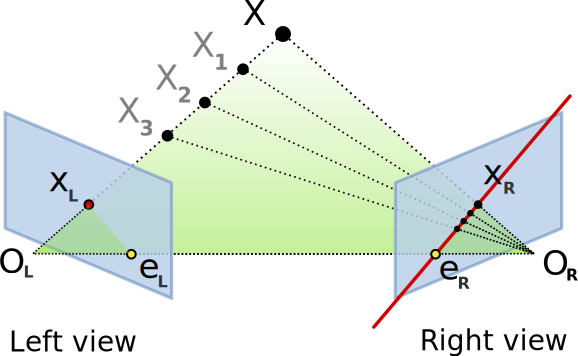
\includegraphics[width=0.4\textwidth]{./images/epipolar_geometry.pdf}
	\end{figure}
	
\end{frame}

\begin{frame}
	\frametitle{Estimación de movimiento}
	\footnotesize
	
	2D-2D
    \begin{columns}
	\begin{column}{0.7\textwidth}
		\begin{itemize}
		\item Error de reproyección:
		\[
		f(\transform{a}{b}, \mapPointsSet)= \sum_{i=1}^{N} \Vert \measurement_{a,i} - \prediction^{\mathrm{s}}(\transform{a}{\worldCoordSystem},\worldPoint_{i}) \Vert^{2} + \Vert \measurement_{b,i} - \prediction^{\mathrm{s}}(\inverse{\transform{a}{b}}\transform{a}{\worldCoordSystem},\worldPoint_{i}) \Vert^{2}
		\]
		\item Algoritmos lineales: 8-point, 5-point
		\end{itemize}
	\end{column}
	\begin{column}{0.3\textwidth}
	    \begin{figure}
			\def\svgwidth{\columnwidth}
			\import{./images/}{tracking_reprojection_error_after.pdf_tex}
		\end{figure}
	\end{column}
\end{columns}

	3D-2D
    \begin{columns}
	\begin{column}{0.7\textwidth}
		\begin{itemize}
			\item Error de reproyección:
			\[
			f(\transform{\worldCoordSystem}{a}, \mapPointsSet)= \sum_{i=1}^{N} \Vert \measurement_{a,i} - \prediction(\inverse{\transform{\worldCoordSystem}{a}},\worldPoint_{i}) \Vert^{2}
			\]
			\item Algoritmos lineales: DLT, PnP
		\end{itemize}
	\end{column}
	\begin{column}{0.3\textwidth}
		\begin{figure}
			\def\svgwidth{\columnwidth}
			\import{./images/}{tracking_reprojection_error_after.pdf_tex}
		\end{figure}
	\end{column}
	\end{columns}
	3D-3D
	\begin{columns}
		\begin{column}{0.7\textwidth}
			\begin{itemize}
				\item Error de reproyección:
				\[
				f(\transform{a}{b})= \sum_{i=1}^{N} \Vert \pointCoord{a}_{i} - \transform{a}{b} \pointCoord{b}_{i} \Vert^{2}
				\]
				\item Algoritmos lineales: Atun, Horn
			\end{itemize}
		\end{column}
		\begin{column}{0.3\textwidth}
			\begin{figure}
				\def\svgwidth{\columnwidth}
				\import{./images/}{tracking_reprojection_error_after.pdf_tex}
			\end{figure}
		\end{column}
	\end{columns}

\end{frame}

\begin{frame}
	\frametitle{Estimación de movimiento 2D-2D}
	\footnotesize
	
	\begin{itemize}
		\item dados los matches 2D-2D $\{(\measurement_{a}, \measurement_{b})_{i}\}$ de puntos 3D desconocidos $\mapPointsSet_{i}$ encontrar el movimiento relativo $\transform{a}{b}$ entre los frames.
		\item Error de reproyección (Bundle Adjustment):
		\[
		f(\transform{a}{b}, \mapPointsSet)= \sum_{i=1}^{N} \Vert \measurement_{a,i} - \prediction^{\mathrm{s}}(\transform{a}{\worldCoordSystem},\worldPoint_{i}) \Vert^{2} + \Vert \measurement_{b,i} - \prediction^{\mathrm{s}}(\inverse{\transform{a}{b}}\transform{a}{\worldCoordSystem},\worldPoint_{i}) \Vert^{2}
		\]
		Se puede optimizar con métodos no lineales pero requieren de una buena semilla inicial. Es no convexo, solución no única (ambigüedadad de escala)
		\item Se puede utilizar un enfoque algebraico basado en geometría epipolar para obtener la transformación relativa (a un factor de escala) sin explicitamente computar la posición de los puntos 3D: algoritmos 8-point y 5-point.
		\item Aplicaciones:
		\begin{itemize}
			\item Filtrar matches con RANSAC
			\item Inicializar una sistemas de SLAM monocular / SfM
		\end{itemize}
	\end{itemize}
\end{frame}

\begin{frame}
	\frametitle{Estimación de movimiento 3D-2D}
	\footnotesize
	
	\begin{itemize}
		\item Dado un conjunto de correspondencias 3D-2D $\{(\worldPoint, \measurement_{a})_{i}\}$ queremos encontrar la pose $\transform{w}{a}$ de la cámara en el mundo.
		\item Error de reproyección:
		\[
		f(\transform{\worldCoordSystem}{a}, \mapPointsSet)= \sum_{i=1}^{N} \Vert \measurement_{a,i} - \prediction(\inverse{\transform{\worldCoordSystem}{a}},\worldPoint_{i}) \Vert^{2}
		\]
		Se puede optimizar con métodos no lineales pero requieren de una buena semilla inicial. Es no convexo, solución no única (ambigüedad de escala)
		\item Este problema es conocido como \emph{Perspective-n-Points} (PnP) y existen diferentes enfoques para resolverlo:
		\begin{itemize}
			\item Direct Linear Transform (DLT)
			\item EPnP
			\item OPnP
		\end{itemize}
		\item Aplicaciones:
		\begin{itemize}
			\item Localización de una cámara dado un mapa de puntos (tracking)
		\end{itemize}
	\end{itemize}
	
\end{frame}

\begin{frame}
	\frametitle{Estimación de movimiento 3D-3D}
	\footnotesize
	
	\begin{itemize}
		\item Dado un conjunto de correspondencias 3D-2D $\{(\worldPoint, \measurement_{a})_{i}\}$ queremos encontrar la pose $\transform{w}{a}$ de la cámara en el mundo.
		\item Error de reproyección:
		\[
		f(\transform{\worldCoordSystem}{a}, \mapPointsSet)= \sum_{i=1}^{N} \Vert \measurement_{a,i} - \prediction(\inverse{\transform{\worldCoordSystem}{a}},\worldPoint_{i}) \Vert^{2}
		\]
		Se puede optimizar con métodos no lineales pero requieren de una buena semilla inicial. Es no convexo, solución no única (ambigüedad de escala)
		\item Este problema es conocido como \emph{Perspective-n-Points} (PnP) y existen diferentes enfoques para resolverlo:
		\begin{itemize}
			\item Direct Linear Transform (DLT)
			\item EPnP
			\item OPnP
		\end{itemize}
		\item Aplicaciones:
		\begin{itemize}
			\item Localización de una cámara dado un mapa de puntos (tracking)
		\end{itemize}
	\end{itemize}
	
	
\end{frame}

\begin{frame}
	\frametitle{Estimación de movimiento 2D-2D}
	\footnotesize
	
\end{frame}



\section{Optical Flow}
  \begin{frame}
  \frametitle{Material para Optical Flow}
  
  \url{https://docs.opencv.org/3.4/d4/dee/tutorial_optical_flow.html}
  \url{https://youtu.be/lnXFcmLB7sM}
  \url{https://www.baeldung.com/cs/motion-field-optical-flow}
  \url{https://rpg.ifi.uzh.ch/docs/teaching/2020/11_tracking.pdf}
  \url{https://rpg.ifi.uzh.ch/teaching.html}
  \url{https://asl.ethz.ch/education/lectures/autonomous_mobile_robots/spring-2021.html}
  \url{https://cs.brown.edu/courses/cs143/2011/results/proj5/gen/}
  \url{https://rpg.ifi.uzh.ch/docs/teaching/2025/03_camera_calibration.pdf}
  \url{https://webdocs.cs.ualberta.ca/~vis/courses/CompVis/lectures13pdf/Lec04OptFlowMot.pdf}
  \url{https://courses.cs.washington.edu/courses/cse576/19sp/notes/Motion19.pdf}

  Flower Garden sequence: \url{https://persci.mit.edu/demos/jwang/garden-layer/orig-seq.html}

  \url{https://cseweb.ucsd.edu/classes/sp19/cse152-a/lec16.pdf}

\end{frame}

\begin{frame}
  \frametitle{Motion Field vs Optical Flow}
  Cuando un objeto se mueve en la escena y es capturado por una cámara, este se proyecta sobre el plano del imagen creando un moviemiento en el plano de la imagen una imagen, al que llamaremos el Motion Field correspondiente a ese punto 3D en movimiento. Desafortunadamente, no es posible garantizar que podamos medir este motion field, todo lo que podemos medir es el movimiento del patrón de brillo en la image, y este se llama Optical Flow.

\end{frame}

% Slide 1
\begin{frame}
  \frametitle{Optical Flow}
  \note{https://youtu.be/lnXFcmLB7sM}

  Method to estimate apparent motion of scene points from a sequence of images.

  Optical flow is the pattern of apparent motion of image objects between two consecutive frames caused by the movement of object or camera. It is 2D vector field where each vector is a displacement vector showing the movement of points from first frame to second.

  Method to estimate the apparent motion of scene points from a sequence of images i.e., the motion of brightness pattern in the image. Each pixel has a vector that tells the optical flow at that point. The motion of the brightness pattern is the optical flow, the length of the vector tells how fast it is moving, and the direction tells its direction on the image plane.

\begin{columns}
  \begin{column}{0.5\textwidth}
    \begin{center}
      \movie[showcontrols,autostart,loop,poster]{\includegraphics[width=0.8\columnwidth]{images/optical_flow/klt_points_video.jpg}}{videos/klt_points.mp4}
      \end{center}
  \end{column}
  \begin{column}{0.5\textwidth}  %%<--- here
    \begin{center}
      \movie[showcontrols,autostart,loop,poster]{\includegraphics[width=\columnwidth]{images/optical_flow/klt_tracking_video.jpg}}{videos/klt_tracking.mp4}
    \end{center}
  \end{column}
\end{columns}

Topics:
\begin{enumerate}
\item Motion Field and Optical Flow
\item Optical Flow Constraint Equation
\item Lucas-Kanade Method
\item Coarse-to-Fine Flow Estimation
\item Applications of Optical Flow
\end{enumerate}
\end{frame}


% Slide 2
\begin{frame}
  \frametitle{Motion Field}
  \begin{center}
    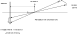
\includegraphics[width=\columnwidth]{./images/optical_flow/motion_field.pdf}
  \end{center}

\end{frame}


\begin{frame}
  \frametitle{Optical Flow}
Motion of brightness patterns in the image.

Ideally: Optical Flow = Motion Field.

\vspace{0.5cm}
\centering
% \includegraphics[width=0.6\textwidth]{placeholder-slide6.png}
\end{frame}

% Slide 4
\begin{frame}
  \frametitle{When is Optical Flow $\neq$ Motion Field?}


  \begin{figure}[!h]
    \subfloat[Motion field]
    {
        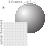
\includegraphics[valign=b,width=0.3\columnwidth]{./images/optical_flow/spinning_sphere_stationary_light.pdf}
    }
    \hspace*{2em}
    \subfloat[Optical Flow]
    {
        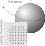
\includegraphics[valign=b,width=0.3\columnwidth]{./images/optical_flow/stationary_sphere_moving_light.pdf}
    }
  \end{figure}

\begin{itemize}
  \item Motion Field exists but no Optical Flow (e.g., spinning sphere, stationary light source)
  \item No Motion Field exists but there is Optical Flow (e.g., stationary sphere, moving light source)
\end{itemize}

\end{frame}

% Slide 3
\begin{frame}
  \frametitle{Optical Flow}
Motion of brightness patterns in the image.

Ideally: Optical Flow = Motion Field.

\vspace{0.5cm}
\centering
% \includegraphics[width=0.6\textwidth]{placeholder-slide6.png}
\end{frame}

% Slide 4
\begin{frame}
  \frametitle{When is Optical Flow $\neq$ Motion Field?}
  \begin{figure}[!h]
    \subfloat[Barber Pole Illusion]
    {
      \movie[showcontrols,autostart,loop,poster]{\includegraphics[valign=m,width=0.2\columnwidth]{./images/optical_flow/barberpole_video.jpg}}{videos/barberpole.mp4}
    }
    \hspace*{2em}
    \subfloat[Motion field]
    {
        
\includegraphics[valign=m,width=0.11\columnwidth]{./images/optical_flow/barberpole_motion_field.pdf}
    }
    \hspace*{2em}
    \subfloat[Optical Flow]
    {
        
\includegraphics[valign=m,width=0.11\columnwidth]{./images/optical_flow/barberpole_optical_flow.pdf}
    }
  \end{figure}
  \begin{itemize}
    \item Barber Pole Illusion: Motion Field horizontal, Optical Flow appears vertical.
  \end{itemize}
\end{frame}

% Slide 4
\begin{frame}{Point Tracking}
  Problem: given two images, estimate the motion of a pixel point from image $I_0$ to image $I_1$
  
  \begin{center}
    \includegraphics[width=0.3\columnwidth]{./images/optical_flow/point_tracking_1.pdf}
  \end{center}

\end{frame}

% Slide 5
\begin{frame}{Point Tracking}
  Problem: given two images, estimate the motion of a pixel point from image $I_0$ to image $I_1$
  
  \begin{center}
    \includegraphics[width=0.3\columnwidth]{./images/optical_flow/point_tracking_2.pdf}
  \end{center}
\end{frame}

% Slide 6
\begin{frame}{Point Tracking}
  \begin{itemize}
    \item Problem: given two images, estimate the motion of a pixel point from image $I_0$ to image $I_1$
  \end{itemize}

  \begin{center}
    \includegraphics[width=0.3\columnwidth]{./images/optical_flow/point_tracking_3.pdf}
  \end{center}
  
  \begin{itemize}
    \item Two approaches exist, depending on the amount of motion between the frames:
      \begin{itemize}
        \item Block-based methods
        \item Differential methods
      \end{itemize}
  \end{itemize}

\end{frame}

% Slide 7
\begin{frame}{Point Tracking}
  Consider the motion of the following corner
  
  \begin{center}
    \includegraphics[width=0.3\columnwidth]{./images/optical_flow/point_tracking_block_matching_1.pdf}
  \end{center}
\end{frame}

% Slide 8
\begin{frame}{Point Tracking}
  Consider the motion of the following corner
  
  \begin{center}
    \includegraphics[width=0.3\columnwidth]{./images/optical_flow/point_tracking_block_matching_2.pdf}
  \end{center}
\end{frame}

% Slide 9
\begin{frame}{Point Tracking with Block Matching}
  \begin{itemize}
    \item Search for the corresponding patch in a $D \times D$ region around the point to track.
    \item Use SSD, SAD, or NCC.
  \end{itemize}
  
  \begin{center}
    \includegraphics[width=0.3\columnwidth]{./images/optical_flow/point_tracking_block_matching_3.pdf}
  \end{center}
\end{frame}

% Slide 10
\begin{frame}{Pros and Cons of Block Matching}
  \textbf{Pros:}
  \begin{itemize}
    \item Works well if the motion is large
  \end{itemize}
  
  \textbf{Cons:}
  \begin{itemize}
    \item Can become computationally demanding if the motion is large
    \item Can the “search” be implemented in a smart way if the motion is “small”?  
      Yes, use Differential methods
  \end{itemize}
\end{frame}

% Slide 11
\begin{frame}{Point Tracking with Differential Methods}
  Looks at the local brightness changes at the same location. No patch shift is performed!
  
  \begin{center}
    \includegraphics[width=0.3\columnwidth]{./images/optical_flow/point_tracking_differential_methods_1.pdf}
  \end{center}
\end{frame}

% Slide 12
\begin{frame}{Point Tracking with Differential Methods}
  Looks at the local brightness changes at the same location. No patch shift is performed!
  
  \begin{center}
    \includegraphics[width=0.3\columnwidth]{./images/optical_flow/point_tracking_differential_methods_2.pdf}
  \end{center}
\end{frame}

% Slide 13
\begin{frame}{Point Tracking with Differential Methods}
  Looks at the local brightness changes at the same location. No patch shift is performed!
  
  \begin{center}
    \includegraphics[width=0.3\columnwidth]{./images/optical_flow/point_tracking_differential_methods_3.pdf}
  \end{center}
\end{frame}

% Slide 14
\begin{frame}{Point Tracking with Differential Methods}
  Assumptions:

  \begin{columns}
    \begin{column}{0.7\textwidth}
      \begin{itemize}
        \item Brightness constancy: The intensity of the pixels around the point to track does not change much between the two frames
        \item Temporal consistency: The motion displacement is small (1–2 pixels); can be addressed using multi-scale implementations
        \item Spatial coherency: Neighboring pixels undergo similar motion (they all lay on the same 3D surface, i.e., no depth discontinuity)
    \end{itemize}
    \end{column}
    \begin{column}{0.3\textwidth}  %%<--- here
      \begin{center}
      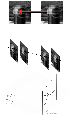
\includegraphics[width=0.7\columnwidth]{./images/optical_flow/point_tracking_differential_methods_properties.pdf}
      \end{center}
    \end{column}
  \end{columns}

\end{frame}


\begin{frame}
  \frametitle{Point Tracking with Differential Methods}
  \begin{figure}[!h]
    \subfloat[]
    {
    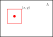
\includegraphics[width=0.4\columnwidth]{./images/optical_flow/klt_displacement_1.pdf}
    }
    \hspace*{2em}
    \subfloat[]
    {
    
\includegraphics[width=0.4\columnwidth]{./images/optical_flow/klt_displacement_2.pdf}
    }
  \end{figure}

  \begin{center}
    Displacement: $(\delta x, \delta y)$ \hspace*{2em} Optical Flow: $(u,v) = \left(\dfrac{\delta x}{\delta t}, \dfrac{\delta y}{\delta t}\right)$
  \end{center}

\end{frame}


\begin{frame}
  \frametitle{Point Tracking with Differential Methods}

  \begin{figure}[!h]
    \subfloat[]
    {
    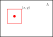
\includegraphics[width=0.4\columnwidth]{./images/optical_flow/klt_displacement_1.pdf}
    }
    \hspace*{2em}
    \subfloat[]
    {
    
\includegraphics[width=0.4\columnwidth]{./images/optical_flow/klt_displacement_2.pdf}
    }
  \end{figure}

  Assumpion \#1:
  Brightness of image point remains constant over time

  \begin{equation*}
    I(x + \delta x, y + \delta y, t + \delta t) = I(x, y, t)
  \end{equation*}

\end{frame}

\begin{frame}
  \frametitle{Taylor Series Expansion}

  Expand a function as an infinite sum of its derivatives

  \[
  f(x + \delta x) = f(x) + \frac{\partial f}{\partial x}\delta x + 
  \frac{\partial^2 f}{\partial x^2}\frac{\delta x^2}{2!} + \cdots + 
  \frac{\partial^n f}{\partial x^n}\frac{\delta x^n}{n!}
  \]

  If $\delta x$ is small:

  \[
  f(x + \delta x) = f(x) + \frac{\partial f}{\partial x}\delta x + 
  \boxed{O(\delta x^2)} \rightarrow \text{Almost Zero}
  \]

  For a function of three variables with small $\delta x, \delta y, \delta t$:

  \[
  f(x + \delta x, y + \delta y, t + \delta t) \approx f(x, y, t) + 
  \frac{\partial f}{\partial x}\delta x + 
  \frac{\partial f}{\partial y}\delta y + 
  \frac{\partial f}{\partial t}\delta t
  \]
\end{frame}


\begin{frame}
  \frametitle{Point Tracking with Differential Methods}

  \begin{figure}[!h]
    \subfloat[]
    {
    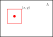
\includegraphics[width=0.4\columnwidth]{./images/optical_flow/klt_displacement_1.pdf}
    }
    \hspace*{2em}
    \subfloat[]
    {
    
\includegraphics[width=0.4\columnwidth]{./images/optical_flow/klt_displacement_2.pdf}
    }
  \end{figure}

  Assumpion \#2:
  Displacement $(\delta x, \delta y)$ and time step $\delta t$ are small
  (Aplicamos taylor)
  \begin{equation*}
    I(x + \delta x, y + \delta y, t + \delta t) = I(x, y, t) + \dfrac{\partial I}{\partial x} \delta x + \dfrac{\partial I}{\partial y} \delta y + \dfrac{\partial I}{\partial t} \delta t
  \end{equation*}


  \begin{equation*}
    \boxed{I(x+\delta x, y+\delta y, t+\delta t) \approx I(x,y,t) + I_x \delta x + I_y \delta y + I_t \delta t}
  \end{equation*}
\end{frame}

\begin{frame}
  \frametitle{Optical Flow Constraint Equation}

  \begin{equation}\label{eq:uno}
    I(x + \delta x, y + \delta y, t + \delta t) = I(x, y, t)
  \end{equation}
  \begin{equation}\label{eq:dos}
    I(x + \delta x, y + \delta y, t + \delta t) = I(x, y, t) + I_x \delta x + I_y \delta y + I_t \delta t
  \end{equation}
  Subtract \eqref{eq:uno} from \eqref{eq:dos}: \quad 
  \[
  I_x \delta x + I_y \delta y + I_t \delta t = 0
  \]
  Divide by $\delta t$ and take limit as $\delta t \rightarrow 0$: \quad 
  \[
  I_x \frac{\partial x}{\partial t} + I_y \frac{\partial y}{\partial t} + I_t = 0
  \]

  Constraint Equation: \quad \boxed{I_x u + I_y v + I_t = 0} \quad $(u,v)$: Optical Flow

  \[
  (I_x, I_y, I_t) \text{ can be easily computed from two frames}
  \]

\end{frame}

%------------------------------------------------
\begin{frame}
  \frametitle{Computing Partial Derivatives $I_x, I_y, I_t$}

  \begin{center}
    
\includegraphics[width=0.35\columnwidth]{./images/optical_flow/computing_partial_derivatives.pdf}
  \end{center}
  %
  \[
  I_x(k, l, t) = \frac{1}{4} [I(k+1,l,t) + I(k+1,l,t+1) + I(k+1,l+1,t) + I(k+1,l+1,t+1)]
  \]
  \[
  - \frac{1}{4}[I(k,l,t) + I(k,l,t+1) + I(k,l+1,t) + I(k,l+1,t+1)]
  \]

  Similarly find $I_y(k,l,t)$ and $I_t(k,l,t)$

\end{frame}

\begin{frame}
  \frametitle{Geometric Interpretation}

  \begin{columns}
    \begin{column}{0.6\textwidth}  %%<--- here
      For any point $(x,y)$ in the image, its optical flow $(u,v)$ lies on the line:
      \[
      I_x u + I_y v + I_t = 0
      \]

      Optical Flow can be split into two components.

      \[
      \mathbf{u} = \mathbf{u}_n + \mathbf{u}_p
      \]

      $\mathbf{u}_n$: Normal Flow \\
      $\mathbf{u}_p$: Parallel Flow
    \end{column}
    \begin{column}{0.4\textwidth}
      \begin{center}
        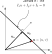
\includegraphics[width=\columnwidth]{./images/optical_flow/optical_flow_geometric_interpretation.pdf}
      \end{center}
    \end{column}
  \end{columns}
\end{frame}

\begin{frame}
  \frametitle{Normal Flow}

  \begin{columns}
    \begin{column}{0.6\textwidth}  %%<--- here
      Direction of Normal Flow:

      Unit vector perpendicular to the constraint line:
      \[
      \hat{\mathbf{u}}_n = \frac{(I_x, I_y)}{\sqrt{I_x^2 + I_y^2}}
      \]

      Magnitude of Normal Flow:

      Distance of origin from the constraint line:
      \[
      |\mathbf{u}_n| = \frac{|I_t|}{\sqrt{I_x^2 + I_y^2}}
      \]

      \[
      \boxed{\mathbf{u}_n = \frac{|I_t|}{(I_x^2 + I_y^2)} (I_x, I_y)}
      \]
    \end{column}
    \begin{column}{0.4\textwidth}
      \begin{center}
        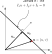
\includegraphics[width=\columnwidth]{./images/optical_flow/optical_flow_geometric_interpretation.pdf}
      \end{center}
    \end{column}
  \end{columns}

\end{frame}

\begin{frame}
  \frametitle{Aperture Problem}

  \begin{itemize}
    \item<1-2> Consider the motion of the following corner
    \item<3-> Now, look at the local brightness changes through a small aperture
    \item<5-> We cannot always determine the motion direction. Infinite motion solutions may exist!
    \item<6-> We can only detect the normal flow.
  \end{itemize}

  \begin{center}

    \only<1>{\includegraphics[width=0.35\columnwidth]{./images/optical_flow/aperture_problem_frame_1.pdf}}

    \only<2>{\includegraphics[width=0.35\columnwidth]{./images/optical_flow/aperture_problem_frame_2.pdf}}

    \only<3>{\includegraphics[width=0.35\columnwidth]{./images/optical_flow/aperture_problem_frame_1_covered.pdf}}

    \only<4>{\includegraphics[width=0.35\columnwidth]{./images/optical_flow/aperture_problem_frame_2_covered.pdf}}

    \only<5>{\includegraphics[width=0.35\columnwidth]{./images/optical_flow/aperture_problem_infinite_motion.pdf}}

    \only<6>{
\includegraphics[width=0.35\columnwidth]{./images/optical_flow/aperture_problem_normal_flow.pdf}}

    \only<7>{\includegraphics[width=0.35\columnwidth]{./images/optical_flow/aperture_problem_actual_motion.pdf}}

  \end{center}
\end{frame}

\begin{frame}
  \frametitle{Aperture Problem}
  \begin{figure}[!h]
    \subfloat[]
    {
      \movie[showcontrols,autostart,loop,poster]{\includegraphics[valign=b,width=0.2\columnwidth]{./images/optical_flow/barberpole_illusion_video.jpg}}{videos/barberpole_illusion.mp4}
    }
    \hspace*{2em}
    \subfloat[]
    {
      \movie[showcontrols,autostart,loop,poster]{\includegraphics[valign=b,width=0.2\columnwidth]{./images/optical_flow/barberpole_aperture_problem_video.jpg}}{videos/barberpole_aperture_problem.mp4}
    }
  \end{figure}
  \begin{itemize}
    \item The aperture problem. The grating appears to be moving down and to the right, perpendicular to the orientation of the bars. But it could be moving in many other directions, such as only down, or only to the right. It is impossible to determine unless the ends of the bars become visible in the aperture.
  \end{itemize}
\end{frame}

% Slide 5
\begin{frame}
  \frametitle{Motion Illusions}

  \TODO{agregar imágenes}

  \begin{itemize}
    \item Donguri Wave Illusion: Static image but perceived motion.
    \item Ouchi Pattern: Inner disc appears to move with respect to the ring.
  \end{itemize}

  \vspace{0.5cm}
  \centering
  % \includegraphics[width=0.6\textwidth]{placeholder-slide9.png}
\end{frame}

% Slide 9
\begin{frame}
  \frametitle{Normal Flow and Aperture Problem}
  \begin{itemize}
    \item Constraint equation gives only a line in $(u,v)$ space.
    \item Can compute normal flow but not full optical flow.
    \item Locally, humans also perceive only normal flow (aperture problem).
  \end{itemize}

  \vspace{0.5cm}
  \centering
  % \includegraphics[width=0.6\textwidth]{placeholder-slide22.png}
\end{frame}

\begin{frame}
    \frametitle{Block-based vs Differential methods}
    
    \begin{itemize}
        \item \textbf{Block-based methods:}
        \begin{itemize}
            \item \textbf{Robust to large motions}
            \item Can be computationally \textbf{expensive} ($D \times D$ validations need to be made for a single point to track)
        \end{itemize}
    \end{itemize}

    \vspace{0.5em} % Adds some vertical space

    \begin{itemize}
        \item \textbf{Differential methods:}
        \begin{itemize}
            \item Works only for \textbf{small motions} (e.g., high frame rate). For larger motion, multi-scale implementations are used but are more expensive (see later)
            \item \textbf{Much more efficient than block-based methods.} Thus, can be used to track the motion of every pixel in the image (i.e., optical flow). It avoids searching in the neighborhood of the point by analyzing the local intensity changes (i.e., differences) of an image patch at a specific location (i.e., no search is performed)
        \end{itemize}
    \end{itemize}

\end{frame}

%------------------------------------------------
\begin{frame}
  \frametitle{Optical Flow is Under Constrained}

  Constraint Equation: \quad \boxed{I_x u + I_y v + I_t = 0}

  \vspace{0.5cm}
  2 unknowns, 1 equation.

  \vspace{1cm}
  We need additional constraints.

\end{frame}

%------------------------------------------------
\begin{frame}
  \frametitle{Lucas-Kanade Solution}

  \textbf{Assumption}: For each pixel, assume Motion Field, and hence Optical Flow $(u,v)$, is constant within a small neighborhood $W$.

  % \begin{center}
  % \includegraphics[width=0.55\textwidth]{placeholder}
  % \end{center}

  That is for all points $(k,l) \in W$:
  \[
  I_x(k,l)u + I_y(k,l)v + I_t(k,l) = 0
  \]

\end{frame}

%------------------------------------------------
\begin{frame}
  \frametitle{Lucas-Kanade Solution}

  For all points $(k,l) \in W$: \quad 
  $I_x(k,l)u + I_y(k,l)v + I_t(k,l) = 0$

  Let the size of window $W$ be $n \times n$

  In matrix form:

  \begin{equation*}
    \underset{\substack{\mathbf{A^T A} \\ \text{(Known)} \\2\times2}}{
    \boxed{
    \begin{bmatrix}
      I_x(1,1) & I_y(1,1) \\
      I_x(k,l) & I_y(k,l) \\
      \vdots & \vdots \\
      I_x(n,n) & I_y(n,n)
    \end{bmatrix}
    }}
    \underset{\substack{\mathbf{u} \\ \text{(Unknown)}\\ 2\times1}}{
    \boxed{
    \begin{bmatrix}
      u \\
      v
    \end{bmatrix}
    }}
    =
    \underset{\substack{\mathbf{B} \\ \text{(Unknown)}\\ n^{2}\times1}}{
    \boxed{
      \begin{bmatrix}
      -I_t(1,1) \\
      -I_t(k,l) \\
      \vdots \\
      -I_t(n,n)
      \end{bmatrix}
    }}
  \end{equation*}


  $n^2$ Equations, 2 Unknowns: Find Least Squares Solution

\end{frame}

%------------------------------------------------
\begin{frame}
  \frametitle{Least Squares Solution}

  Solve linear system: \quad $\mathbf{A u = B}$

  \begin{equation*}
  \mathbf{A^T A u = A^T B} \hspace{1cm} \text{(Least-Squares using Pseudo-Inverse)}
  \end{equation*}

  In matrix form:

  \begin{equation*}
  \underset{\substack{\mathbf{A^T A} \\ \text{(Known)} \\2\times2}}{
    \boxed{
    \begin{bmatrix}
    \sum_W I_x I_x & \sum_W I_x I_y \\
    \sum_W I_x I_y & \sum_W I_y I_y
    \end{bmatrix}
    }
  }
  \underset{\substack{\mathbf{u} \\ \text{(Unknown)}\\ 2\times1}}{
    \boxed{
      \begin{bmatrix}
      u \\ v
      \end{bmatrix}
    }
  }
  =
  \underset{\substack{\mathbf{A^T B} \\\text{(Known)} \\ 2\times1}}{
    \boxed{
      \begin{bmatrix}
      -\sum_W I_x I_t \\ -\sum_W I_y I_t
      \end{bmatrix}
    }
  }
  \qquad \substack{\text{Indices} (k,l)\\ \text{not written}\\ \text{for simplicity}}
  \end{equation*}

  \begin{equation*}
  \boxed{\mathbf{u} = (\mathbf{A^T A})^{-1}\mathbf{A^T B}}
  \end{equation*}

  Fast and Easy to Solve

\end{frame}

% Slide 12
\begin{frame}
  \frametitle{Large Motion: Problem}
Taylor approximation invalid when displacements are large.

\vspace{0.5cm}
\centering
% \includegraphics[width=0.6\textwidth]{placeholder-slide34.png}
\end{frame}

% Slide 13
\begin{frame}
  \frametitle{Coarse-to-Fine Estimation}
Use resolution pyramid:
\begin{itemize}
  \item Compute flow at low resolution.
  \item Warp and refine at higher resolutions.
  \item Repeat until full resolution.
\end{itemize}

\vspace{0.5cm}
\centering
% \includegraphics[width=0.6\textwidth]{placeholder-slide36.png}
\end{frame}

% Slide 14
\begin{frame}
  \frametitle{Alternative Approach: Template Matching}
\begin{itemize}
  \item Use template window from one frame.
  \item Search for best match in next frame.
  \item Difference gives optical flow.
  \item Slow and can produce mismatches.
\end{itemize}

\vspace{0.5cm}
\centering
% \includegraphics[width=0.6\textwidth]{placeholder-slide41.png}
\end{frame}

% Slide 15
\begin{frame}
  \frametitle{Applications of Optical Flow}
\begin{itemize}
  \item Optical mouse: motion tracking.
  \item Traffic monitoring: estimate vehicle speed.
  \item Video retiming: slow motion.
  \item Stabilization: remove camera shake.
  \item Face tracking: expressions, blinking.
\end{itemize}

\vspace{0.5cm}
\centering
% \includegraphics[width=0.6\textwidth]{placeholder-slide47.png}
\end{frame}

% References
% \begin{frame}
%   \frametitle{References}
%     \tiny
%     [Barron 2005] J. L. Barron, D. J. Fleet, and S. Beauchemin, IJCV 2005. \\
%     [Black 1993] M. J. Black and P. Anandan, ICCV 1993. \\
%     [Bouguet 2000] J. Y. Bouguet, Intel Tech Report 2000. \\
%     [Brox 2004] T. Brox, A. Bruhn, N. Papenberg, J. Weickert, ECCV 2004. \\
%     [Horn 1981] B. K. P. Horn and B. G. Schunck, AI 1981. \\
%     [Liu 2014] S. Liu, L. Yuan, P. Tan, J. Sun, CVPR 2014. \\
%     [Lucas 1981] B. D. Lucas and T. Kanade, Imaging Workshop 1981.
% \end{frame}

\section{Bibliografía}
\section{Bibliografía}
\begin{frame}
    \frametitle{Bibliografía}
    \nocite{siegwart2011introduction}
    \nocite{corke2017robotics}
    \nocite{hartley2003multiple}
    \nocite{misra2006global}

    \printbibliography

\end{frame}
	
\end{document}